\documentclass[12pt,letterpaper,english,bibliography=totocnumbered, abstract=on]{scrartcl}

\usepackage{indentfirst}
\usepackage[titletoc]{appendix}
\usepackage[T1]{fontenc}
\usepackage[latin9]{inputenc}
\usepackage{color}
\usepackage{babel}
\usepackage{verbatim}
\usepackage[unicode=true,pdfusetitle,
bookmarks=true,bookmarksnumbered=false,bookmarksopen=false,
breaklinks=true,pdfborder={0 0 0},pdfborderstyle={},backref=false,colorlinks=true]
{hyperref}
\hypersetup{linkcolor=blue,citecolor=blue,urlcolor=blue}

\usepackage{booktabs}
\usepackage{multirow}
\usepackage{adjustbox}
\usepackage{threeparttable}
\usepackage[table]{xcolor}
\usepackage{csquotes}
\usepackage{soul} % for hiliting text: \hl

\usepackage[backend=biber, style=authoryear, maxbibnames=99, dashed=false]{biblatex}
\setlength\bibitemsep{2\itemsep}
\addbibresource{CRB.bib}

\usepackage{pdfpages}
\usepackage{float} % Allows use of H to place floats

\usepackage{pgfgantt}

\usepackage{framed}

% Prevent page breaks within paragraphs
% https://tex.stackexchange.com/questions/21983/how-to-avoid-page-breaks-inside-paragraphs
\widowpenalties 1 10000

\begin{document}

%\titlehead{Titlehead}

\title{Data Analysis for CRB Trap Improvement Article}

\author{Aubrey Moore}

\date{\today}


\maketitle

\tableofcontents

\footnote{The most recent version of this document can be downloaded from\\
\url{https://github.com/aubreymoore/CRB-trap-improvement/blob/master/results.pdf}.}

\pagebreak

\section{Depleted Lures}

asasas \cite{moore_research_2012}

\section{Trap Catch Summary}

\begin{table}[h]
	\caption{Caption goes here.}
	\tiny
	\centering
	\begin{tabular}{@{}llccccc@{}}
		\toprule
		Trap type & \multicolumn{1}{c}{Description} & \multicolumn{3}{c}{Beetles trapped} & \begin{tabular}[c]{@{}c@{}}Proportion of\\traps which caught\\one or more beetles\\during 2 week\\trapping periods\end{tabular} & \begin{tabular}[c]{@{}c@{}}Beetles caught\\per trap-day\\(mean $\pm$ SEM)\end{tabular} \\ \midrule
		&  & Male & Female & Total &  &  \\ \cmidrule(lr){3-5}
		T & \begin{tabular}[c]{@{}l@{}}Trap with no lure\\ and no UVLED\end{tabular} & 0 & 0 & 0 & 0/36 & 0.000 $\pm$ 0.000 \\
		T-UV & \begin{tabular}[c]{@{}l@{}}Trap with no lure\\ and UVLED\end{tabular} & 0 & 2 & 2 & 2/36 & 0.003 $\pm$ 0.002 \\
		T-RL & \begin{tabular}[c]{@{}l@{}}Trap with reduced release\\ rate lure\end{tabular} & 9 & 4 & 13 & 7/36 & 0.027 $\pm$ 0.012 \\
		T-SL & \begin{tabular}[c]{@{}l@{}}Trap with standard release\\ rate lure\end{tabular} & 11 & 9 & 20 & 10/36 & 0.039 $\pm$ 0.014 \\
		T-UV-RL & \begin{tabular}[c]{@{}l@{}}Trap with reduced release\\ rate lure and UVLED\end{tabular} & 18 & 20 & 38 & 12/36 & 0.073 $\pm$ 0.025 \\
		T-UV-SL & \begin{tabular}[c]{@{}l@{}}Trap with standard release\\  rate lure and UVLED\end{tabular} & 30 & 24 & 54 & 15/36 & 0.109 $\pm$ 0.031 \\ \bottomrule
	\end{tabular}
\end{table}

\begin{figure}[h]
\centering
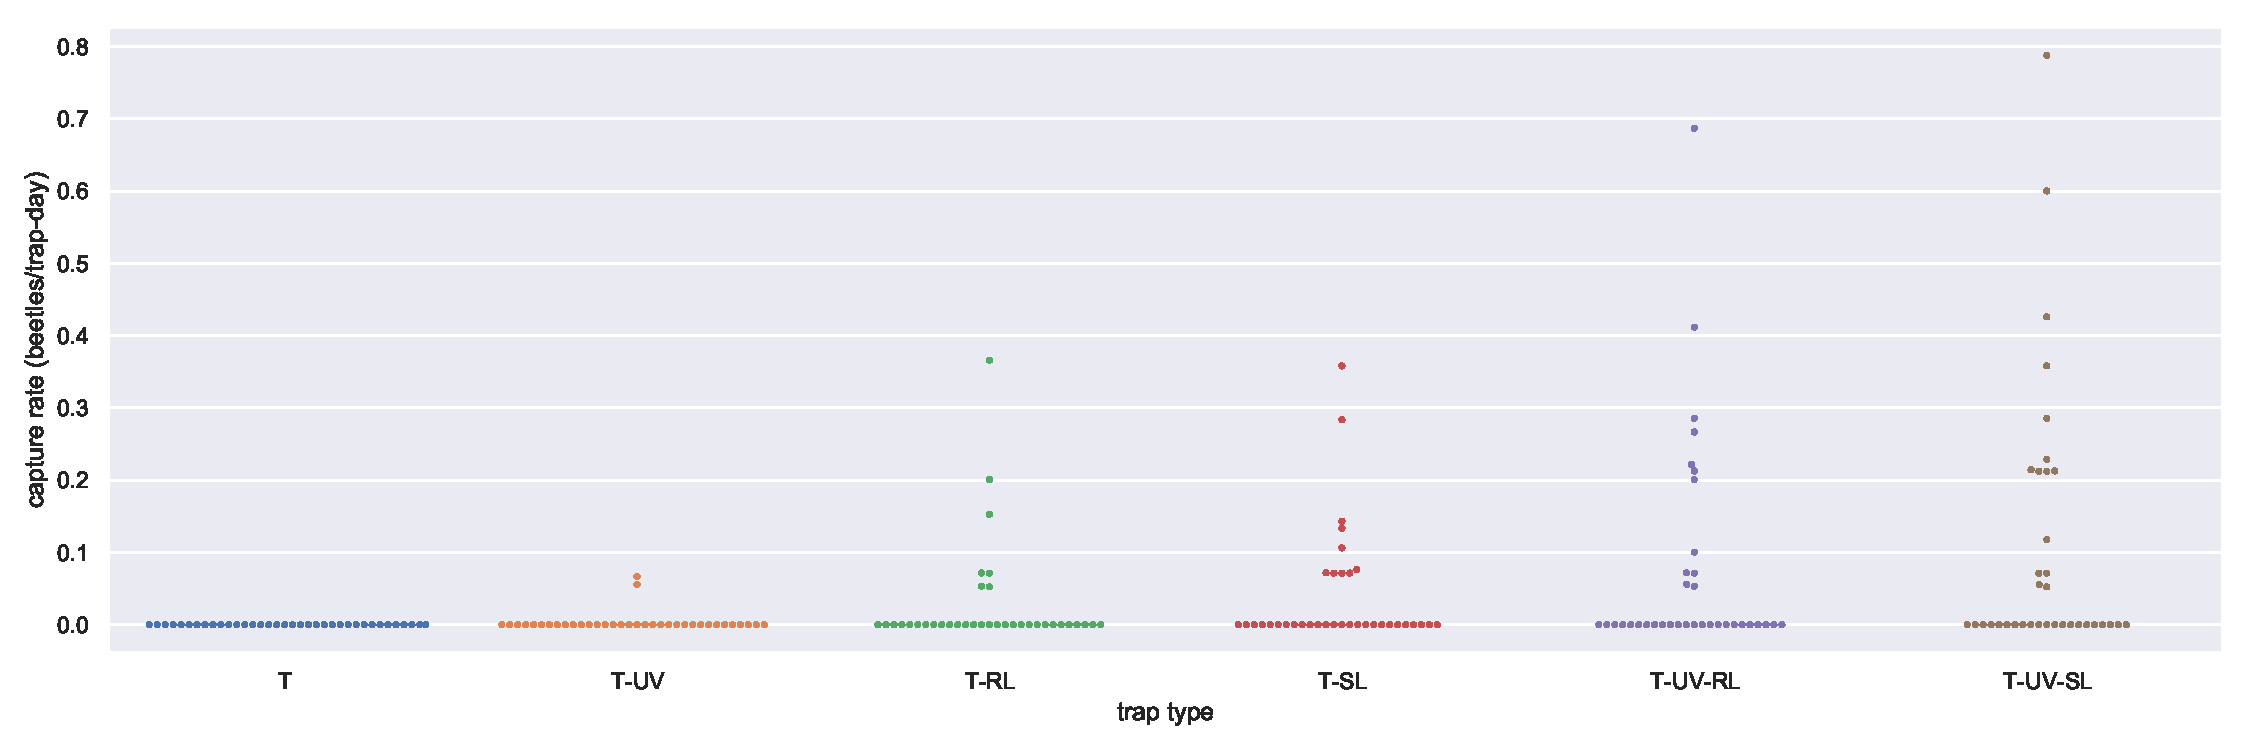
\includegraphics[width=1\linewidth]{images/trapcatch-swarmplot}
\caption{Swarm plot.}
\label{fig:trapcatch-swarmplot}
\end{figure}

\newpage

\section{Capture Rate as a Function of Pheromone Release Rate}

\begin{figure}[h]
\centering
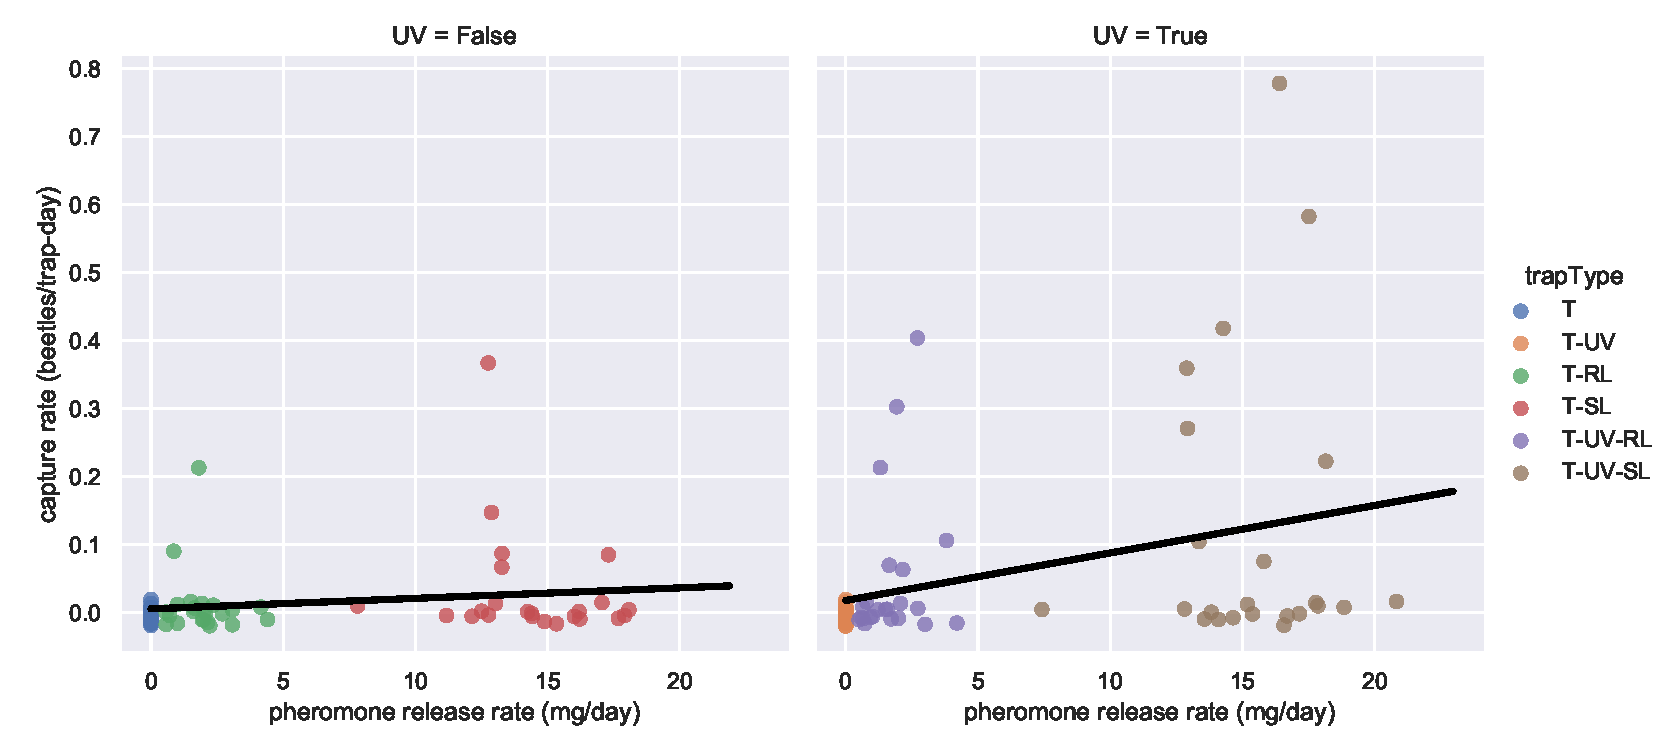
\includegraphics[width=1\linewidth]{images/trapcatch-lmplot}
\caption{Caption.}
\label{fig:trapcatch-lmplot}
\end{figure}

\printbibliography	

\end{document}
